\documentclass[conf]{new-aiaa}
%\documentclass[journal]{new-aiaa} for journal papers
\usepackage[utf8]{inputenc}

\usepackage{graphicx}
\usepackage{amsmath}
\usepackage[version=4]{mhchem}
\usepackage{siunitx}
\usepackage{longtable,tabularx}
\setlength\LTleft{0pt} 

% my packages
\usepackage{wrapfig}
\usepackage{float}
\usepackage{subfigure}

\title{Interaction of Geomagnetic Storms on Earth Magnetic Anomaly Navigation}

\author{Spencer A. Freeman}
\affil{Virginia Tech, Blacksburg, VA, 24061}

\begin{document}

\maketitle

\begin{abstract}
The topic of this report is the interaction of geomagnetic storms on Earth magnetic anomaly navigation. The Earth’s magnetic field can be decomposed into subcomponents based on the source of each component. The greatest contributor is known as the core field, which is generated by the Earth's perpetually circulating molten iron core. This field is on the order of 30,000 – 50,000 nanoteslas (nT). A much smaller contributor is known as the Earth Magnetic Anomaly which is generated by induced magnetization of materials in the Earth’s crust. This field is on the order of 100’s of nT. The core field varies only over long ranges whereas the magnetic anomaly varies much greater spatially and thus provides a viable candidate signal for local navigation. Unfortunately, there are time varying components in the magnetic field that are much more difficult to predict. The ionosphere creates induced magnetic fields through the circulation of ions. This is exacerbated by solar interference which creates more ions, and thus unpredictable magnetic disturbances which corrupt the magnetic anomaly readings. This report details a study on the navigational impacts of these disturbances.
\end{abstract}

\section{Outline and Key Aspects}
\lettrine{T}{his} report is a study on the interaction of geomagnetic storms on Earth magnetic anomaly navigation. The methodology was to simulate a Kalman filter updated with simulated magnetometer measurements and observe the results under different magnetospheric conditions. Several items needed to be developed to perform the simulation.\\

\begin{enumerate}
   \item Acquire magnetic anomaly map
   \item Generate truth trajectory
   \item Develop magnetometer sensor model
        \begin{description}[font=$\bullet$\scshape\bfseries]
            \item Acquire geomagnetic storm data
            \item Implement storm data into magnetometer model
        \end{description}
   \item Create Kalman filter simulation 
       \begin{description}[font=$\bullet$\scshape\bfseries]
            \item Implement magnetometer measurement update
        \end{description}
   \item Plot and interpret results\\
\end{enumerate}

This first step was to acquire data for use in the simulation. Magnetic anomaly navigation requires a precise map of the local magnetic field which is used to relate measurements to geodetic location. Most anomaly maps are localized and do not share a common format due to their genesis in the natural resource prospecting industry. Some attempts have been made to produce global maps which combine existing data; For the purposes of this project, the National Oceanic and Atmospheric Administration (NOAA) Earth Magnetic Anomaly Grid 2-arc-minute resolution (EMAG2) v3 dataset will serve this purpose. In addition to serving as the geodetic map, EMAG2 was used to generate simulated magnetometer measurements with noise added mimicking real world data. Lastly, data representing the effects of geomagnetic storms on the magnetic field was needed. Given the randomness of their occasions, these effects are most reliably captured by persistent ground based sensors. The British Geological Survey maintains a web service called INTERMAGNET, which hosts magnetometer data recorded at dozens of sites around the world [CITE]; data from the USGS Fredericksburg, VA station was pulled for use in this project.

The key aspect of this project is studying the ability of the navigation system to handle time-varying biases in the magnetic anomaly field measurement. Since the physical sensor measures the total field strength, which is the summation of multiple components, the measurement must be processed to extract the value of the magnetic anomaly field. Geomagnetic storms induce temporary magnetic fields around the Earth which disturb the permanent magnetic field. Even given warning of solar activity, the localized effects are difficult to predict and time-varying, so accounting for the disturbances presents a challenge.

This project presents these effects by perturbing measurements of the permanent magnetic field with actual recorded data from known geomagnetic storms. In recent memory, a Coronal Mass Ejection in February 2022 produced a storm that caused global disruption including the loss of 38 commercial satellites [CITE]. The magnetic effects of this event were seen even at ground level via recording stations across the world. The data from one of these stations was used to mimic the time-varying disturbances the would likely be observed by a sensor at some location.  

\section{Background} % ==========================================

In order to motivate the study of magnetic disturbances on navigation, a review of navigation algorithms and the physics of the Earth's magnetic field is necessary. A brief, but thorough description of navigation algorithms will be presented along with the chosen architecture for this analysis. The principles of geodetic navigation are simple enough, but their practical implementation is generally quite intricate and nuanced. A simplified model will be used to analyze the topic at hand. Additionally, a review of Earth's magnetic field and the models used to describe it are presented in just enough detail to allow discussion of their use as navigation signals.

\subsection{Geodetic Navigation} % -----------------------

Navigation is the method of determining position, course, and distance traveled of some vehicle [CITE - https://www.merriam-webster.com/dictionary/navigation]. Generally defined by a global frame of reference, navigation with respect to the Earth can be considered geodetic. Some examples of this practice are global navigation satellite systems (GNSS) which use RF transmissions and precise timing to geolocate receivers. The process of navigation utilizes signals which encode information about the state of a vehicle to estimate the state or some subspace of states. Part of the process is rejection of noise, which is unavoidable in any practical navigation signal. The quintessential algorithm for state estimation is the Kalman filter, an optimal solution for filtering of noisy signals. Derivations of the Kalman filter equations are given in [CITE bar shalom]. Sparing the full derivation, the discrete-time implementation is given here. The Kalman filter is a two-step procedure:\\

\begin{enumerate}
    \item Propagate state estimate and covariance.
        \begin{description}[font=$\bullet$\scshape\bfseries]
            \item \(\overline{x} = \Phi \hat{x}\)
            \item \(\overline{P} = \Phi P \Phi^{T} + Q\)
        \end{description}
    \item Update state estimate and covariance using the measurement.
        \begin{description}[font=$\bullet$\scshape\bfseries]
            \item \(M = (M^{-1} + H^{T}R^{-1}H)^{-1}\)
            \item \(K = PH^{T}R^{-1}\)
            \item \(\hat{x} = \overline{x} + K(z - \overline{z})\) \\
        \end{description}
\end{enumerate}

The first step propagates the state estimate and state covariance given a dynamics model encoded in the state transformation matrix \(\Phi\) and process noise \(Q\). The state transformation matrix is a linearization of the system dynamics and the process noise matrix is the covariance of the noise present in the system dynamics. This term captures unmodeled or unknown dynamics and is generally used as a tuning parameter.

The second step is the measurement update. This is where measurements are processed into the state estimate and covariance. Key terms are the measurement-state transformation matrix \(H\) and the measurement covariance matrix \(R\). \(H\) is derived from the generally nonlinear formulation of the measurement as a function of the state; it is a linearization computed analytically or numerically \(H = dz/dx\). \(R\) is the measurement noise covariance and is in practice is estimated from sensor data.

\subsection{Components of Earth's Magnetic Field} % -----------------------

Magnetic fields describe the physical phenomenon of forces exerted on and generated by circulating currents and elementary particles. Magnetic fields are vector fields with magnitude and direction in 3-dimensional space and as with all vector fields, the total value at one point can be decomposed into a sum of sub components. The Earth's magnetic field is that which exists within the Earth extending to the outer magnetosphere several Earth radii outwards. There are several prime contributors to the total field which can be isolated by their source. The component buildup is given in the following equation:

\begin{equation}
    H(x, t) = H_{crust}(x) + H_{core}(x) + H_{ion}(x, t) + H_{other}(x, t), \; (nT)
\end{equation}

\(H_{core}\) is the largest magnitude component in the field. It is generated by the Earth's perpetually circulating, molten iron core which causes circulating electrical currents and thus an astronomically relevant magnetic field at the surface. It is roughly approximated by a dipole and has magnitudes on the  order of 40,000 (nT).

\(H_{ion}\) is the combination of induced magnetic fields caused by currents in the ionosphere. Solar radiation ionizes particles in the atmosphere creating a conductive plasma where electric currents can flow. These currents generate magnetic fields the superimpose onto the observed field spatially and temporally.

\(H_{other}\) is a catch all for unknown or unmodeled disturbances in the field.

\(H_{crust}\) is the component of the field which is generated by induced magnetization of conductive materials in the Earth's crust (lithosphere). This magnetization is latent from induced magnetization from existing fields becoming permanent due to cooling [CITE ]. This component varies in magnitude on the order of 100's of nanteslas and spatially in kilometers. This in conjunction with its time invariant nature (crustal magnetization varies only on geological times scales) makes it a practical candidate for map-based navigation [CITE].  

\subsection{Geomagnetic Storms} % -----------------------

Geomagnetic storms are events in the ionosphere and magnetosphere which cause above average electrical currents which in turn create disturbances in the quiet time magnetic field. They are driven by high intensity solar winds emitted by the sun for short periods which generate ions that circulate in the ionosphere creating induced currents \cite{Physics_of_the_Earths_Space_Environment}. These events can be triggered by Solar Flares or Coronal Mass Ejections (CME) originating from the Sun's surface.

\section{Data and Methods} % ==========================================

This section will cover the data and methods applied to this study. The conceptual math and physics describing the natural phenomenons has been previously thus far been described; the specific methods relating to the math and physics is the topic of this section. The first section will cover the filter design and simulation methodology, the second section will cover the magnetic field models implemented in the simulation, and last section covers the representation of geomagnetic storms in the simulation. Particular detail will be given to the data sources and their pedigree since they are core to the analysis at hand.

\subsection{The Kalman Filter} % -----------------------

\begin{wrapfigure}{r}{0.4\textwidth} %this figure will be at the right
    \centering
    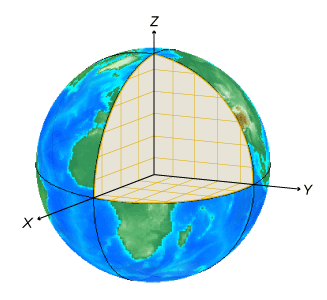
\includegraphics[width=0.4\textwidth]{figures/ecef_system.png}
    \caption{ECEF Coordinates \cite{mathworks_ecef}.}
\end{wrapfigure}

The workhorse of state estimation is the discrete time Kalman filter. There are many flavors of this filter and nearly all are tailored for their specific use case; the level of complexity flows down as needed by the use case. Simpler is always preferred and in the case of real-time estimation, a design requirement due to embedded systems processing limitations. For the purposes of this project, the chosen state model was the 3 Cartesian components of position in the Earth Centered, Earth Fixed (ECEF) frame. A constant acceleration model was used to represent the dynamics which specifies 9 total states for the filter to process; position, velocity, and acceleration of each ECEF component. This is a common coordinate system which works globally and is well standardized in the aerospace field. Constant acceleration implies that the dynamics are assumed to be constant acceleration over each time step. This dictates the form of the state transformation matrix \(\Phi\). 

\begin{equation}
    \Phi = \begin{bmatrix} I_{3x3} & \Delta t & \frac{1}{2}\Delta t^{2} \\ 0_{3x3} & I_{3x3} & \Delta t \\ 0_{3x3} & 0_{3x3} & I_{3x3} \end{bmatrix}
\end{equation}

The discrete time process noise model used in this analysis is simple although the derivation is complicated. It assumes the noise in the dynamics originate solely in the acceleration; there is no direct uncertainty that the derivative of position is velocity. The form of the process noise covariance matrix is given here:

\begin{equation}
    Q = \begin{bmatrix} \frac{1}{2}\Delta t^{5} & \frac{1}{8}\Delta t^{4} & \frac{1}{6}\Delta t^{3} \\ \frac{1}{8}\Delta t^{4} & \frac{1}{3}\Delta t^{3} & \frac{1}{2}\Delta t^{2} \\ \frac{1}{6}\Delta t^{3} & \frac{1}{2}\Delta t^{2} & \Delta t \end{bmatrix}\Tilde{q}
\end{equation}

The filter must be initialized with some a prioi estimate of the state vector and covariance matrix. As long as this data is in the ballpark of the true values, the filter should converge as intended. In this analysis random variations were added to the initial state estimate and the covariance matrix was initialized with the following values:

\begin{equation}
    x_{0} = x_{0_{truth}} + w_{\sigma}
\end{equation}

Where \(w_{\sigma}\) is a 9x1 vector of normally distributed white noise applied at initialization. The first 3 elements are the distribution of positional noise, the next 3 are velocity and last 3 acceleration error. The standard deviation of this noise is given in Table 1 along with other filter parameters. 

\begin{center}
\begin{tabular}{||c c c | c | c||} 
 \hline
 $\sigma_{position}$ & $\sigma_{velocity}$ & $\sigma_{acceleration}$ & $\Tilde{q}$ & $\Delta t$ \\ [0.5ex] 
 \hline
  10 \((m)\) & 2 \((m/s)\) & 0.2 \((m/s^{2})\) & 1 $(m^{2}/s^{5})$ & 1 $(s)$ \\ [1ex] 
 \hline
\end{tabular}
\end{center}

\subsection{Magnetic Field Representation} % -----------------------

With the simple filter design worked out, the next step was to develop a model of the Earth's magnetic field through the buildup of each component as previously discussed. As previously discussed, the signal of interest is the component of the magnetic field produced by minerals in the crust. There are actually 2 data points needed: a measurement of the total field (that which would be observed by a real magnetometer) and a map of the crustal component precisely relating the field magnitude to geodetic position. The maps are built offline by collecting field strength data at known locations; this is very practical using modern GNSS positioning and survey aircraft. The difficulty  The method for simulating this measurement was to simply use the map value (treated as truth) and add appropriate noise to the simulated measurement injected into the filter. This method avoids many of the challenges of magnetic navigation (core field estimation, map integrity, magnetometer dynamics, etc) but keeps the essence intact enough to observe general trends in the techniques applied. The measurement z contains 3 components: the crustal field interpolated from the map, Gaussian white noise, and a time-varying input, which will be discussed in Section \ref{geostorm_rep}. The buildup is summarized in Equation \ref{measurement_buildup}:

\begin{equation} \label{measurement_buildup}
    z(x_{ truth}) = H_{map}(x_{ truth}) + H_{noise} + H_{temporal}(t)
\end{equation}

The predicted field value is generated using the map and the current state estimate. This is the process that would be implemented on a real time system using pre-loaded map data. The effect of the crust on magnetic field is most variable in the plane horizontal to the Earth's surface, but does vary some vertically. There are techniques for processing the vertical component known as upward continuation, but for simplification they are omitted for this analysis. The spatial wavelengths of the crustal field vary roughly with altitude (wavelength = altitude) as a convenient rule of thumb \cite{Absolute_Positioning_Using_the_Earths_Magnetic_Anomaly_Field}. Magnetic navigation has yet to become widespread and so comprehensive high quality maps are not abundant. Most that are sufficient for navigation purposes were created for the natural resource prospecting industry and are thus localized and not standardized. Many lie behind pay walls for the work of creating the maps. Even so, there have been some international efforts to make worldwide magnetic anomaly maps freely available. One example is the NOAA Earth Magnetic Anomaly Grid 2-arc-minute resolution (EMAG2) v3; this map is global in scale, available publicly on the internet \cite{noaa_emag2}. Unfortunately, the EMAG2 as its name implies features data only down to the 2-arc-minute resolution and at only 2 levels: sea level and 4 km above sea level. 2 arc-minutes is ~3.5 km at the equator, meaning only data at that spacing is available. This would not be sufficient for sub kilometer navigation, but can still be used as a signal for less precise positioning and analysis of techniques.

% \begin{figure}[H]
% \centering
% \includegraphics[width=.75\textwidth]{figures/EMAG2_V3_upcontposter.png}
% \caption{EMAG2 v3 \cite{noaa_emag2}}
% \end{figure}

\subsection{Geomagnetic Storm Representation} \label{geostorm_rep} % ------------------

The topics discussed thus far have outlined the basics of magnetic anomaly navigation and a simplified model for simulating a case. The next section describes models needed for the heart of this study: effects of geomagnetic storms on magnetic navigation. Magnetic storms are by nature complex and chaotic processes which are difficult to predict precisely. Thus it was decided to pursue real data as inputs to the simulation. Since storms occur infrequently, most data on magnetic field disturbances are captured by persistent ground based recording stations. These are operated by geophysical science agencies around the world and the collected data is publicly available. Much of this data is hosted by the British Geological Survey and made available through a web service called INTERMAGNET \cite{intramagnet}. The methodology for applying this data to the magnetometer model was to take the recorded data and subtract off the known components specific to that locale. The remaining component should reflect the affect of the temporal (time varying) disturbances. Taking data captured during known geomagnetic storms paints a fairly accurate snapshot of storm effects which could be reasonably applied to other locations. This is summarized in Equations \ref{H_temporal} and \ref{H_ion}.

\begin{equation} \label{H_temporal}
    H_{temporal}(x, t) = H_{crust}(x) + H_{core}(x) + H_{ion}(x, t) + H_{other}(x, t), \; (nT)
\end{equation}

\begin{equation} \label{H_ion}
    H_{ion}(x, t) = H_{temporal}(x, t) - (H_{crust}(x) + H_{core}(x) + H_{other}(x, t)), \; (nT)
\end{equation}

The temporal data was chosen from the closest survey station. Since the region of interest for this analysis is western Virginia, the closest station was the National Geological Survey (NGS) in Fredericksburg, VA (FRD). 

\section{Results} % ==========================================

This section will present the results of the project and describe the data that was generated. Detailed  analysis and conclusions will be reserved for Section \ref{discussion}. The initial results detail the nominal case where no time-varying disturbances are applied. This is the so called, solar quiet (Sq) time where the magnetic field is generally quite predictable on a day to day basis. This is the easiest case for navigation and is thus a good reference point for comparison. The plots following the Sq case will show the results of navigation simulation under geomagnetic storm conditions as modeled by the time-varying storm data discussed previously.

\subsection{Quiet Time} % -----------------------

Since we are most interested in horizontal motion, a projection of the truth trajectory and estimated trajectory are overlaid onto the magnetic field map contour. The truth line is shown as a black dashed line and the estimated line is shown in magenta.

\begin{figure}[H]
\centering
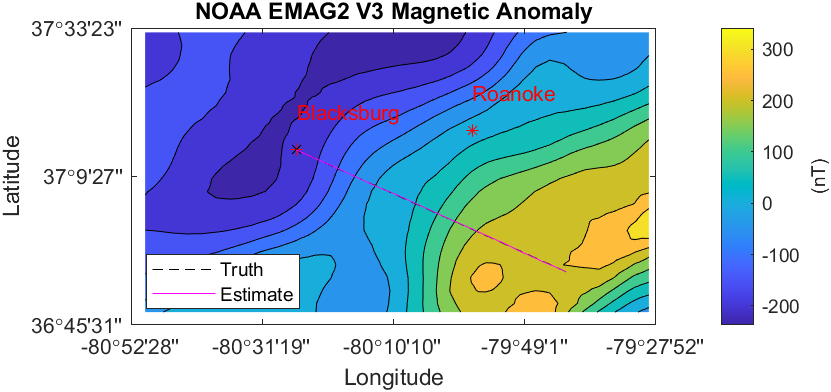
\includegraphics[width=1.0\textwidth]{figures/trajectory_quiet.png}
\caption{Trajectory, Sq.}
\end{figure}

The time history of the filter data is shown in the next plot. This shows the quantitative performance of the state estimation at all points during the trajectory. The data is plotted on a log scale to appropriately capture the spread of data. The 4 time histories are as follows: position error magnitude, velocity error magnitude, acceleration error magnitude, and normalized innovation squared (NIS). The true errors are shown in blue and the covariances (estimated error) are co-plotted in orange.

\begin{figure}[H]
\centering
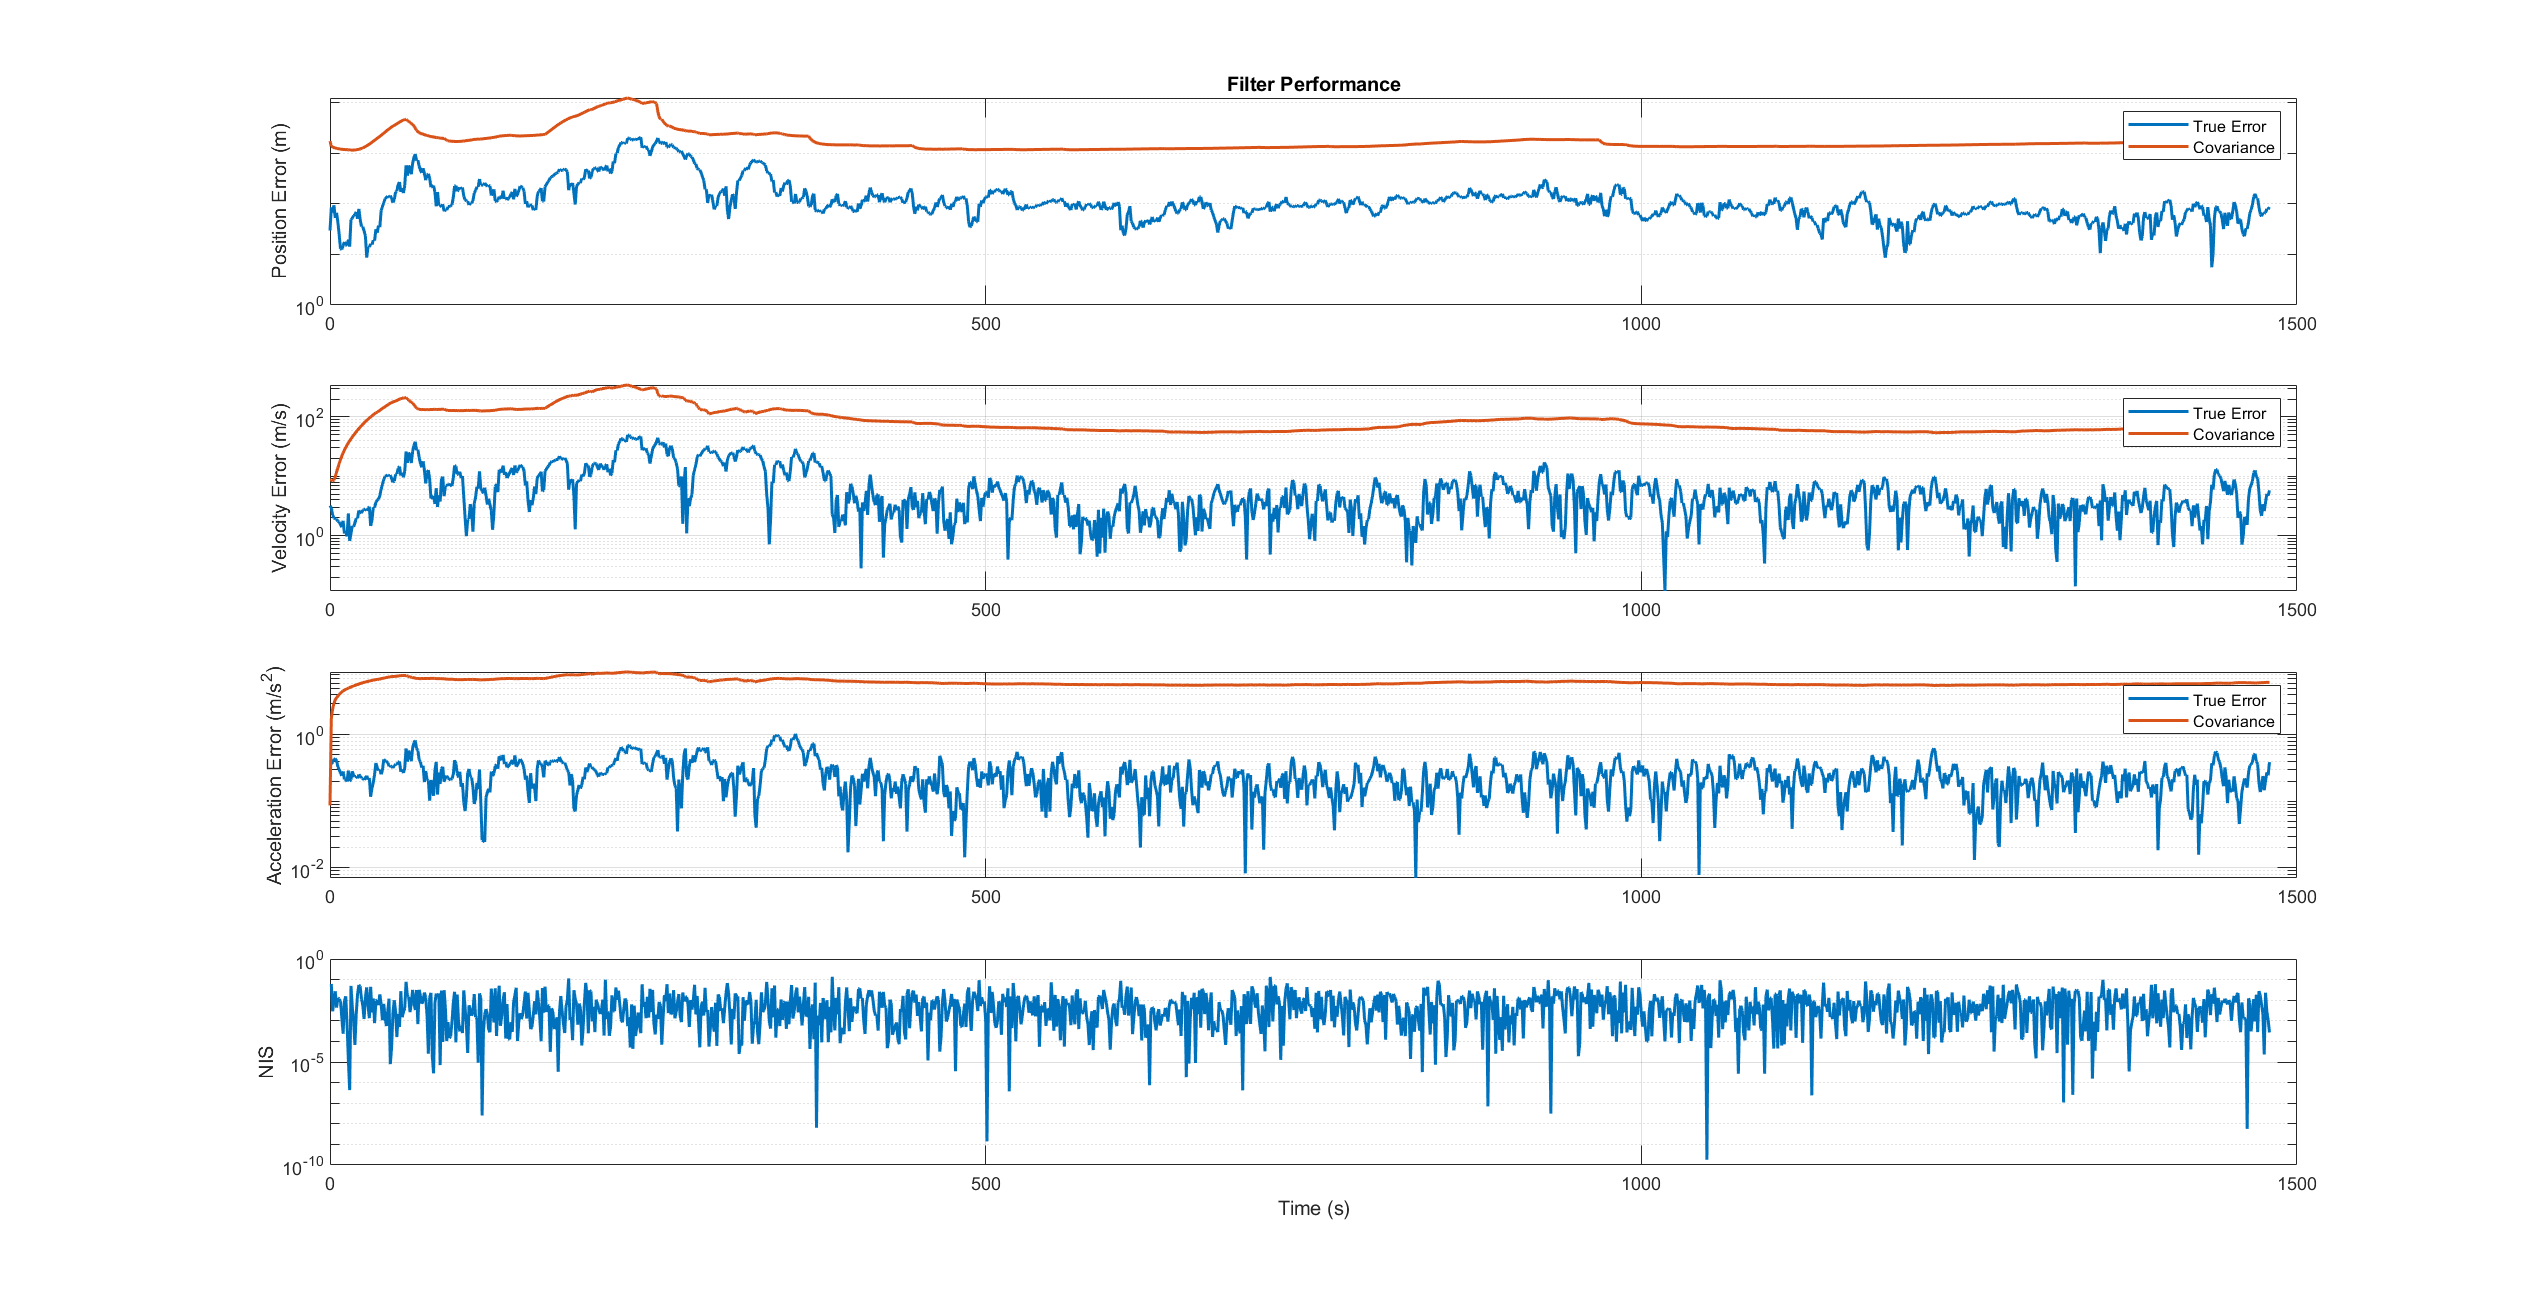
\includegraphics[width=1.0\textwidth]{figures/filter_quiet.png}
\caption{Filter Performance, Sq.}
\end{figure}

As expected, the filter performs quite well; the estimated trajectory nearly hides the true trajectory by lining up exactly. The filter settles nicely early in the trajectory as shown by the steady state of the time histories.

\subsection{Stormy} % -----------------------

This subsection presents the storm time results of the analysis. Before diving into the filter output, a display of the the storm model is warranted. As discussed before, there was a need to pre process the storm data in order to extract the storm effects (remove core field and local magnetic anomaly); this procedure was performed on data from Sq time recorded by the NGS Fredericksburg station. This is shown in the following plots.

\begin{figure}[H]
\hfill
\subfigure[Raw Data]{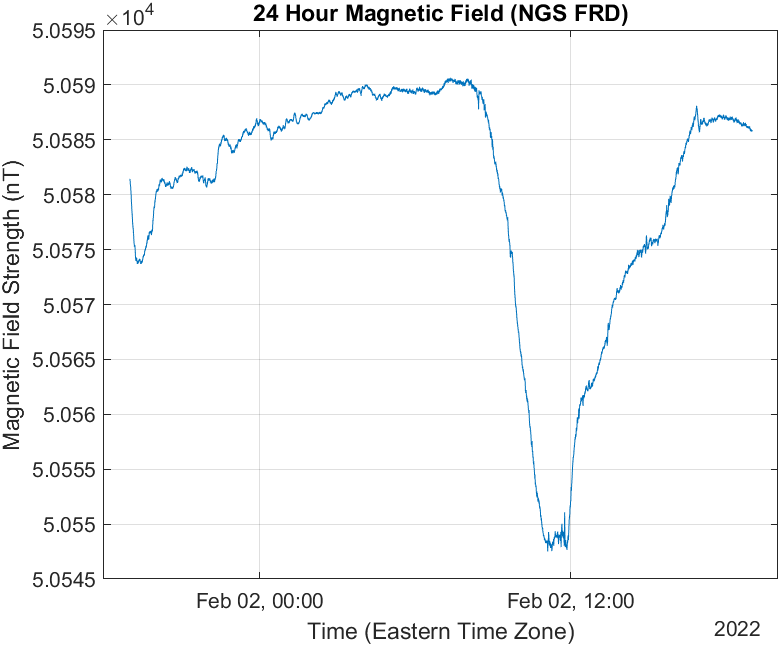
\includegraphics[width=0.4\textwidth]{figures/temporal_sq_raw.png}}
\hfill
\subfigure[Local Effects Removed]{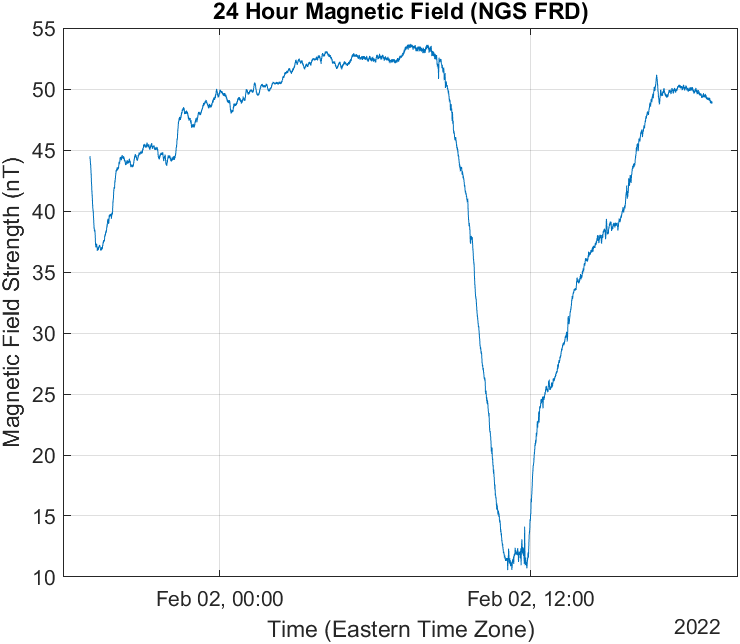
\includegraphics[width=0.4\textwidth]{figures/temporal_sq.png}}
\hfill
% \caption{Title for both}
\end{figure}

This data represents a snapshot of the daily variation in magnetic field activity. Their is a noticeable dip at local noon time which aligns with the understanding of solar activity \cite{Physics_of_the_Earths_Space_Environment}. Since this variation is consistent on a daily basis, it is reasonable that it may be corrected for in the measurement using a time based lookup. To approximate this process, a model was fit to 14 days of 1-minute temporal resolution data that was superimposed and time-averaged. This is shown here:

\begin{figure}[H]
\centering
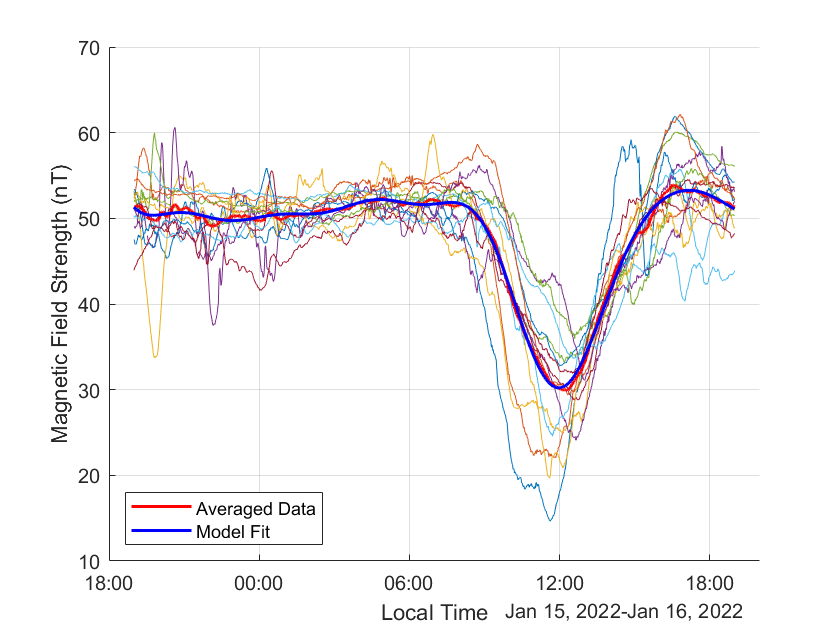
\includegraphics[width=0.85\textwidth]{figures/daily_model_fit.png}
\caption{Daily Variation Fitted Data.}
\end{figure}

Given this predictable variation, the model can be used to correct the measurements using a low complexity approach (model is a sum of 6 sines with fitted weights). This will be more representative approach to a real system and is thus necessary to compare the storm time results with. The results of a simulation with the adjustment applied is shown below.

The estimated temporal variation is overlaid with the true variation in the next plot. It estimates well in the night time but fails largely during daylight.

\begin{figure}[H]
\centering
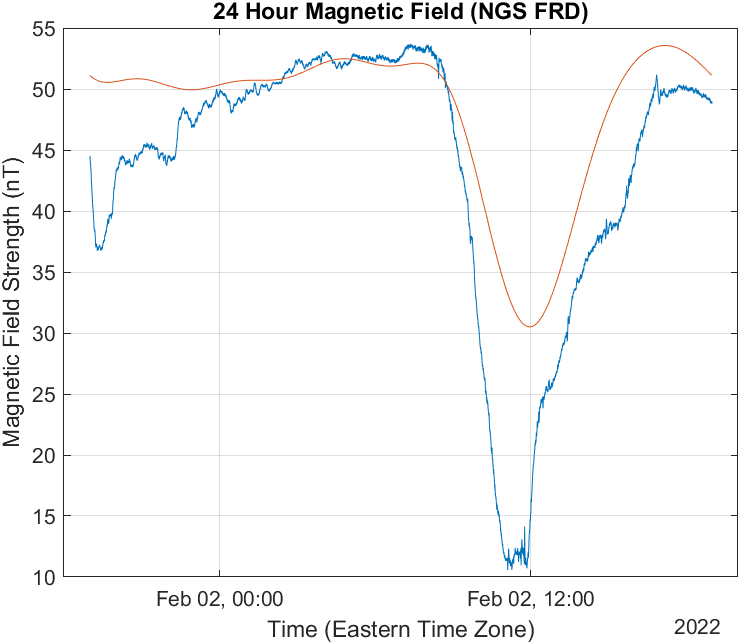
\includegraphics[width=0.75\textwidth]{figures/temporal_sq_and_fit.png}
\caption{Variation with Estimation, Sq.}
\end{figure}

\begin{figure}[H]
\hfill
\subfigure[Trajectory Sq, Daily Variation]{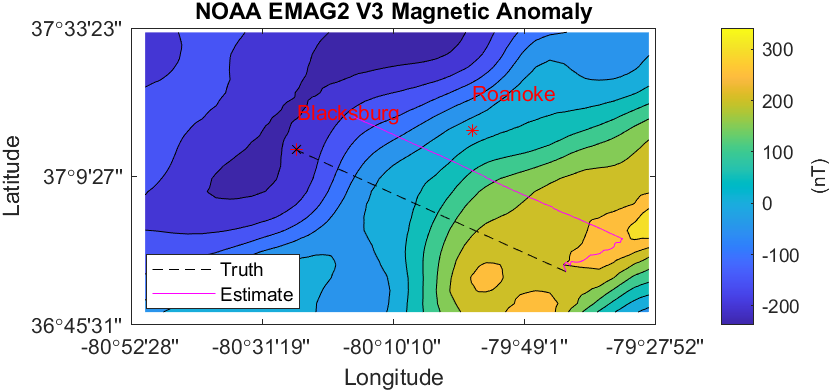
\includegraphics[width=0.45\textwidth]{figures/trajectory_quiet_temporal.png}}
\hfill
\subfigure[Trajectory Sq, Daily Variation Corrected]{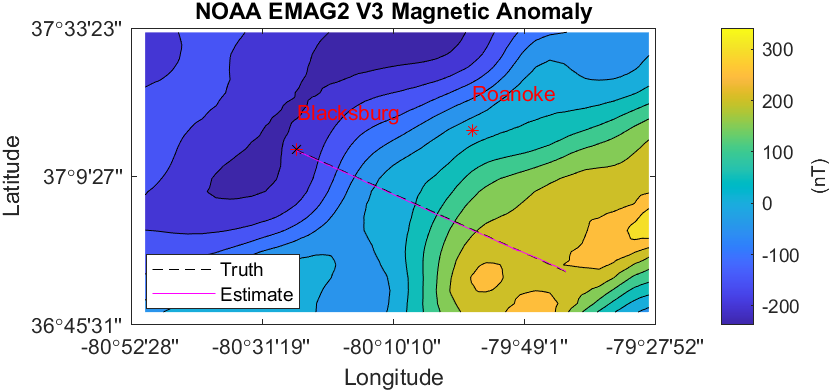
\includegraphics[width=0.45\textwidth]{figures/trajectory_quiet_temporal_corrected.png}}
\hfill
% \caption{Title for both}
\end{figure}

With the daily variation accounted for (not perfect, but close), the simulation of the filter during storm time can be practically compared. The choice of storm data was from the February 3, 2022 geomagnetic storm which was particularly devastating on commercial satellites where 38 satellites were lost. The daily variation shows just how much impact the storm had on magnetic field measurements.

\begin{figure}[H]
\centering
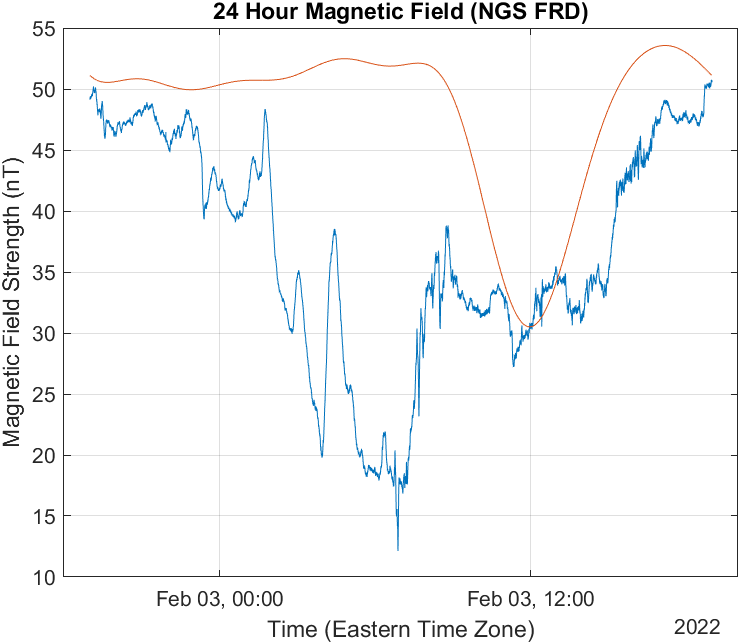
\includegraphics[width=0.75\textwidth]{figures/temporal_storm_and_fit.png}
\caption{Variation with Estimation, Storm.}
\end{figure}

Obviously, the correction assuming the usual daily variation will be hopelessly inaccurate. The ultimate question remains how much error will the filter accumulate due to this inaccuracy. The following plots are the simulation for this storm period.

\begin{figure}[H]
\centering
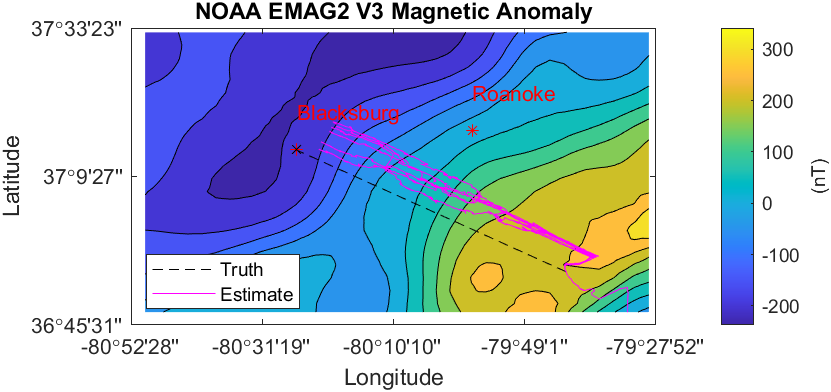
\includegraphics[width=1.0\textwidth]{figures/trajectory_storm_multi.png}
\caption{8 Trajectories, Storm.}
\end{figure}

The previous plot shows 8 runs of the simulation co-plotted. The noise in the system causes each result to diverge from their nominally common initial conditions. Interestingly, they all exhibit a similar bias from the true trajectory; they creep northeasterly uphill with respect to the magnetic anomaly contour before diverging due to integrated errors.

The filter output time history is shown below for 1 case of the batch; the others show similar trends at varying levels of error.

\begin{figure}[H]
\centering
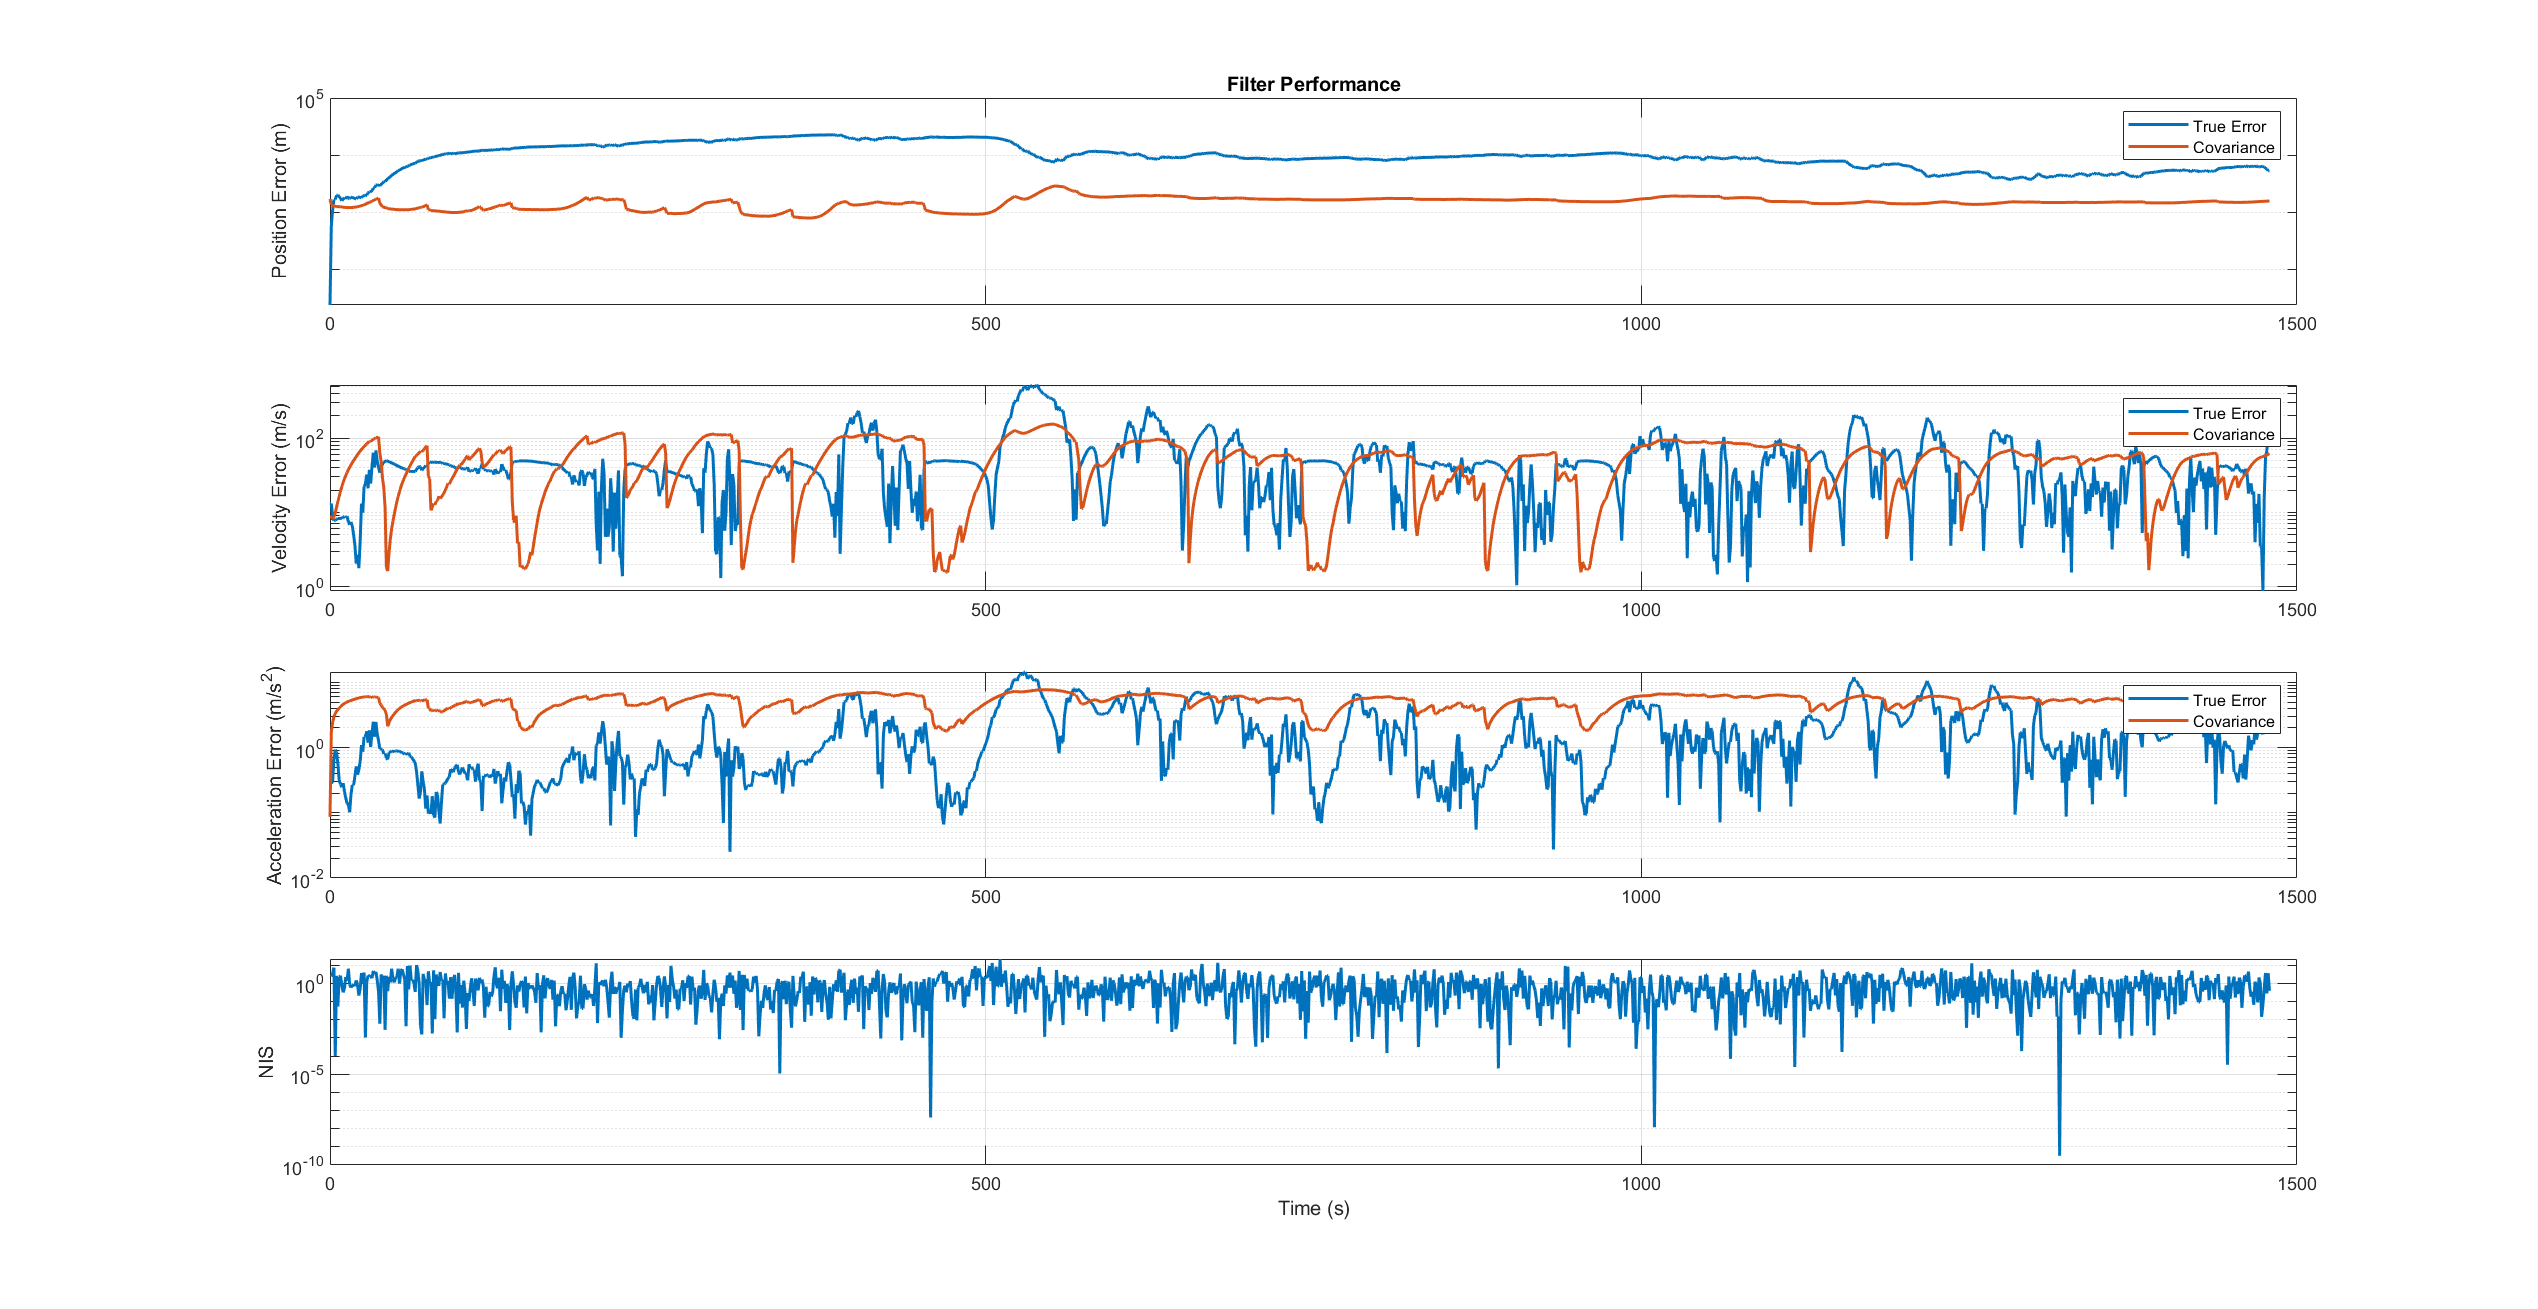
\includegraphics[width=1.0\textwidth]{figures/filter_storm.png}
\caption{1 Select from 8 Trajectories, Storm.}
\end{figure}

\section{Discussion} \label{discussion} % ==========================================



\section{Further Work} % ==========================================

\section*{Appendix} % ==========================================

\bibliography{sample} % ==========================================

\end{document}
